\documentclass[10pt,a4paper]{report}
\usepackage[utf8]{inputenc}
\usepackage[russian]{babel}
\usepackage[OT1]{fontenc}
\usepackage{amsmath}
\usepackage{amsfonts}
\usepackage{amssymb}
\usepackage{graphicx}

\begin{document}
\begin{titlepage}
\title{Описание протокола}
\author{Скрипаль Б.А.}
\end{titlepage}

\chapter{Задание}
Разработать клиент-серверную систему сетевого форума из сервера сетевого форума и пользовательских клиентов.
\section{Основные возможности сервера}
\begin{enumerate}
\item Прослушивание определенного порта
\item Обработка запросов на подключение по этому порту от клиентов
\item Поддержка работы нескольких клиентов через механизм нитей
\item Регистрация подключившегося клиента
\item Выдача клиенту перечня новых сообщений форума
\item Выдача клиенту иерархического представление форума
\item Прием от клиента сообщения в ветку форума
\item Выдача списка текущих активных пользователей форума
\item Обработка запроса на отключения клиента
\item Принудительное отключение клиента
\end{enumerate}
\section{Основные возможности клиента}
\begin{enumerate}
\item Установление соединения с сервером
\item Посылка регистрационных данных клиента
\item Получение и вывод перечня новых сообщений 
\item Получение и вывод иерархии форума
\item Выбор текущей ветки форума
\item Посылка сообщений в текущую ветку форума
\item Разрыв соединения
\item Обработка ситуации отключения клиента сервером
\end{enumerate}
\chapter{Нефункциональные требования}
\section{Требования к реализации}
Соединение начинает сервер, отправляя приглашение к авторизации. Далее клиент пересылает свой логин и пароль. После этого пользователь может просматривать форум (его иерархию и отдельные сообщения), оставлять сообщения в выбранную ветку форума. После завершения работы клиент должен разорвать соединение.
\section{Требования к надежности}
Длинна принимаемого сервером пакета должна быть ограничена, для избежания падения сервера. Так же мы должны обрабатывать неправильные (неккоректные) запросы от клиента.
\section{Накладываемые ограничения}
\begin{enumerate}
\item Ограничение на длинну пакета - все пакеты можно условно разделить на две группы:
\begin{enumerate}
\item Пакеты подтверждения доставки пакета - для данной цели используются пакеты фиксированной длины 2 байта (сообщение "ОК"). Данное сообщение отправляется в качестве подтверждения получения нового сообщения
\item Пакеты содержащие команды пользователя и ответы сервера - в данном случае использовались пакеты длинной 256 символов. Данное ограничение было сделано из следующий соображений: самое длинное (теоретически) сообщение - добавление нового сообщения в форум. Ограничение на длинну сообщения - 150. Команда добавления + разделители занимают суммарно 6 байт. Оставшихся 50 байт (теоретически) должно хватить на задание темы поста.
\end{enumerate}
\item Обрыв сессии (некорректное завершение работы клиентом). При некорректном завершении сессии клиентом он останется в состоянии "online", что является минусом данного протокола.
\item В протоколе отсутствуют возможности создание новой учетной записи, а так же создание новых тем форума.
\end{enumerate}
\chapter{Описание протокола работы}
\section{Описание основных команд пользователя}
\begin{itemize}
\item topics - вывод архитектуры форума в следующем виде: выводится название темы, затем отделенные табуляцией имена "постов" в данной теме с их уникальными идентификаторами.
\item show номер поста - просмотр содержание выбранного поста. При этом в аккаунт пользователя заносится информация о том, что данное сообщение было просмотренно и в дальнейшем оно не будет показываться как новое при авторизации пользователя. Если указать неверный id, то не выводится никакое сообщение.
\item online - вывод списка активных пользователей. Под термином "активный пользователь" понимается пользователь, присутствующий в данный момент на форуме.
\item add Имя темы\&Название поста\&Содержание поста - добавление нового "поста" в выбранную пользователем ветвь форума. Если имя темы указано неверно, то тема не будет добавлена на сетевой форум.
\item exit - завершение сеанса. После ввода данной команды связь между клиентом и сервером обрывается, и пользователь переходит в состояние оффлайн.
\end{itemize}
\section{Диаграмма организации клиент-серверного обмена}
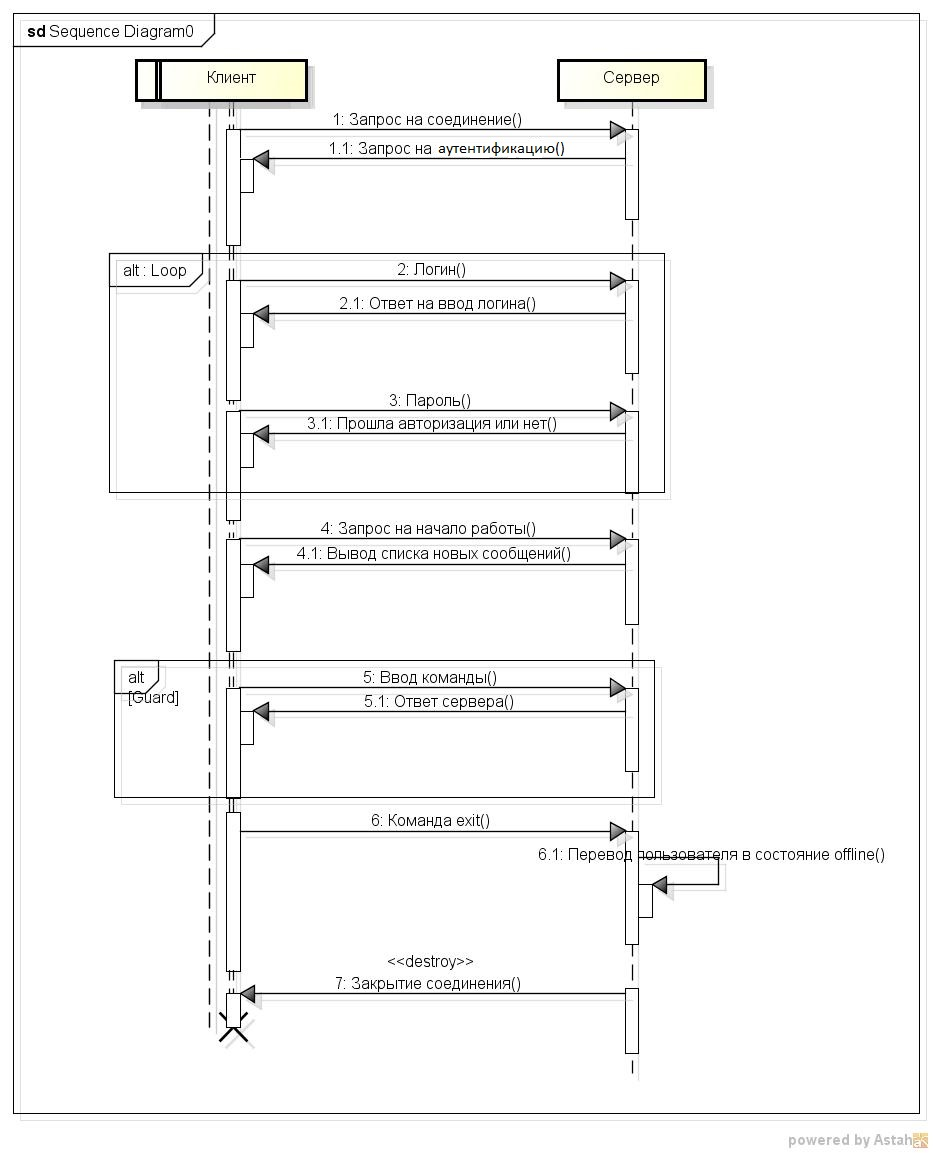
\includegraphics[scale=0.5]{diagram}
\chapter{Архитектура приложения}
\section{Формат хранения данных}
Все данные о пользоветелях, а так же все сообщения форума хранятся в формате XML. К данным о пользователях относится следующее:
\begin{itemize}
\item Уникальный идентификатор пользователя
\item Логин пользователя
\item Пароль пользователя
\item Список просмотренных сообщений
\end{itemize}
Структура форума в представлении XML имеет следующий вид:
\begin{itemize}
\item Каждая тема топика хранится как отдельный тэг. К атрибутам темы относится её имя
\item Внутри каждой темы содержатся список постов форума, относящихся к этой теме. К атрибутам поста отоносится:
\begin{itemize}
\item Уникальный идетнификатор поста
\item Имя поста
\item Содержание сообщения поста
\end{itemize}
\end{itemize}
Для работы с XML-файлами была использована библиотека libxml2. Данная библиотека была выбрана из следующих соображений:
\begin{itemize}
\item Кроссплатформенность - т.к. по заданию было необходимо реализовывать клиентское и серверное приложение под платформы windows и linux, то необходимо что бы используемая библиотека была бы под оба типа операционных систем.
\item Легкость в использовании и большое количество технической документации
\item Надежность
\end{itemize}
В ходе работы приложения используются следующие функции данной библиотеки:
\begin{itemize}
\item Открытие файла для чтения и сохранение изменений в файле
\item Получение потомка
\item Чтение заданных атрибутов потомка, их изменение и сохранение
\end{itemize}
\section{Дизайн протокола}
\begin{itemize}
\item Клиент отправляет серверу сообщение о начале работы 
\item В ответ сервер разрешает работу клиента. На стороне клиента появляется сообщение "Enter login"
\item Клиент вводит свой логин и нажимает клавишу Enter. Логин отправляется серверу, а на стороне клиента появляется приглашение ввести пароль "Enter password"
\item После ввода пароля, если авторизация прошла успешно, то клиенту выводятся новые ("не прочитанные им") сообщения форума, и начинается ожидание новой команды клиента. Причиной неудачи при авторизации могут быть следующие:
\begin{itemize}
\item Неправильная пара логин-пароль. В случае если клиент не может вспомнить пароль или логин и хочет выйти, ему достаточно ввести слово "exit" в поле "логин" и сеанс связи прервется.
\item Данный клиент уже находится в состоянии online на сервере
\end{itemize}
\item При вводе пользователем команды topics ему передается структура сетевого форума, а именно список тем и содержащеися в них посты. Посты отделены от тем знаком табуляции. Так же рядом с каждым сообщением выводится его уникальный идентификатор.
\item Для просмотра содержания выбранного сообщения клиентом вводится команда show, после которой следует номер сообщения, например: "show 00001". В этом случае клиенту выведется содержание данного поста.
\item При вводе команды online клиенту выводится список всех пользователей, которые присутствуют на форуме в данный момент. Каждое имя отделено от другого переносом строки
\item Для добавление нового сообщения используется команда add, после которой следуют имя темы, имя нового сообщения и содержание сообщения. Для отделения каждого из атрибуттов используется знак \&. Например "add Telecom\&Example\&This is test topic". Для того, что бы убедиться в том, что тема добавлена в форум, можно набрать команду topics и увидеть новую тему в списке сообщений.
\item Для завершения сеанса клиенту необходимо ввести команду "exit". После этого сеанс закончится и пользователю будет выведено сообщение о завершении работы.
\end{itemize}
\section{Пример работы с приложением}
\begin{verbatim}
Начало сессии
Hello, print you login and password

Print login

Приглашение на ввод пароля
Print password

Вывод новых сообщений
Hello, telecom!

Hello, telecom again!

Test tcp

Ввод команды topics
topics
Topics:
Telecom
	00001	Why i like telecom
	00001	Why i like telecom
	00002	Hello, telecom!
	00001	Why i like telecom
	00002	Hello, telecom!
	00003	Hello, telecom again!
	00001	Why i like telecom
	00002	Hello, telecom!
	00003	Hello, telecom again!
	36753	Test tcp
Other topic
Ввод команды show
show 00001
Because i must love it

Ввод команды online
online
john

ввод команды add
add Telecom&Test&This is test
Writing
topics
Topics:
Telecom
	00001	Why i like telecom
	00001	Why i like telecom
	00002	Hello, telecom!
	00001	Why i like telecom
	00002	Hello, telecom!
	00003	Hello, telecom again!
	00001	Why i like telecom
	00002	Hello, telecom!
	00003	Hello, telecom again!
	36753	Test tcp
	00001	Why i like telecom
	00002	Hello, telecom!
	00003	Hello, telecom again!
	36753	Test tcp
	36754	Test
Other topic

Ввод команды exit
exit
exit
\end{verbatim}
Так же серверное приложение позволяет организовывать работу нескольких клиентов одновременно. В результате проверки не было выявлено никаких ошибок многопоточности.
\end{document}
